\section{SNMP - Simple Network Management Protocol}
\label{Section:SNMP}

The Simple Network Management Protocol (SNMP) was introduced in 1988 by the  Internet Engineering Task Force (IETF). The reason for this was that at this time, computers got more popular and the need to connect them increased. The result has been that more devices have been included in IP networks. One goal of SNMP was to simplify the management of bigger networks and allow remote management of devices for system administrators, but the main goal was to monitor network components. The protocol was designed to provide a simple set of instructions. The most used implementation for SNMP is called "Net-SNMP"\footnote{\url{http://www.net-snmp.org}} and is available on all major operating systems. Over the years, multiple versions of SNMP have been released, but only three of them are mainly used: v1, v2c, v3. The versions are not backward compatible and the SNMP devices need to implement the detection of the used protocol.

\newpage
The communication between network devices is handled by agents. There is one master agent which communicates with other master agents. The master agent is getting the needed information from other agents on the same device. The agents are exposing data from MIBs (see Section \ref{Section:MIB}) as variables. They also handle a set of instructions, if data in their MIB tables are affected.

The most important features of SNMP are \textit{get}, \textit{set} instructions and \textit{traps}. With the get instruction, it is possible to request data from devices by specifying the OID of the data set. The \textit{set} instruction can modify the data saved on a specified OID. There is also a \textit{walk} instruction, that allows querying multiple OID at once. To accomplish this, the SNMP agent sends multiple \textit{get} requests. There is also an advanced version of \textit{walk}, called \textit{bulkwalk}, that can improve the performance when querying multiple OIDs.

The simplest and first version of SNMP was v1. It has no security mechanisms besides community strings and only supports up to 32-bit counters while the communication is in plain text. In 1993, SNMP v2c was designed, which is a subversion of v2. It introduced an inform command, which is similar to a trap, but with acknowledgments. The focus of v2c has been performance improvements and better error handling. With v3 security mechanisms, encryption and authentication have been introduced.

SNMP is now also used to configure network devices, which is a new purpose for the protocol. Because of this change in use-case, the IEFT introduced a successor standard called NETCONF (see Section \ref{Section:NETCONF}) in 2006. 
Until today, SNMP is still the most used open protocol to configure and monitor network devices. For simplicity, the next sections will only contain the most recent SNMP definitions.

\subsection{Architecture}
The architecture of SNMP is defined in RFC 3411 \cite{RFC:RFC3411:2002}. Its goal is to make SNMP modular to allow evolution over time.

The SNMP management system is a network with multiple devices that can be managed by SNMP. These devices are called SNMP entities and contain a command responder application and a notification originator application. These applications need to have access to management instrumentation, also called agents. The network must contain at least one manager, which is a device that manages other devices. It is an SNMP entity containing a command generator application or a notification receiver application, or both applications can be contained. A compatible management protocol between communicating SNMP entities is needed.

Managers are devices that monitor and control other SNMP entities. They are often implemented on servers or end-user devices for temporary usage. Managed devices are hosts, routers, switches, servers, etc, that are controlled and monitored via their management information base.

\newpage
If a security model is used for SNMP, it should protect against modification of information and masquerade. There should also be protection to prevent message stream modifications and disclosure. A security model does not need to protect against denial of service and traffic analysis. Denial of service floods the network with messages, which results in a failure of the network. In that case, SNMP can not operate anymore. The attack method traffic analysis uses package analysis to predict operations. These predictions are easy due to the design of SNMP. For that reason, it was decided that protection against this attack vector is not needed.

SNMP messages are encapsulated in Protocol Data Units (PDUs). Because SNMP messages can have different use cases, they are classified into seven categories. Every PDU type can be classified into multiple categories. The following classes exist according to RFC 3411 (\cite{RFC:RFC3411:2002}):

\begin{minipage}{\textwidth}
\begin{itemize}
    \item Read Class - For operations that retrieve management information, for example: GetRequest-PDU, GetNextRequest-PDU, and GetBulkRequest-PDU.
    \item Write Class - For operations that modify management information, for example: SetRequest-PDU.
    \item Response Class - For operations which are a response of a previous request, for example: Response-PDU, Report-PDU.
    \item Notification Class - For operations that are sending notifications to a notification receiver, for example: Trapv2-PDU, InformRequest-PDU.
    \item Internal Class - For operations that exchange information between SNMP engines, for example: Report-PDU.
    \item Confirmed Class - For operations that are causing the receiving SNMP engine, to send back an acknowledgment, for example: GetRequest-PDU, GetNextRequest-PDU, GetBulkRequest-PDU, SetRequest-PDU, and InformRequest-PDU.
    \item Unconfirmed Class - For operations that are not causing the sending of an acknowledgment, for example: Report-PDU, Trapv2-PDU, and GetResponse-PDU.
\end{itemize}
\end{minipage}


\subsubsection{SNMP Entity}
\label{Section:SNMP-Entity}

\begin{figure}[!ht]
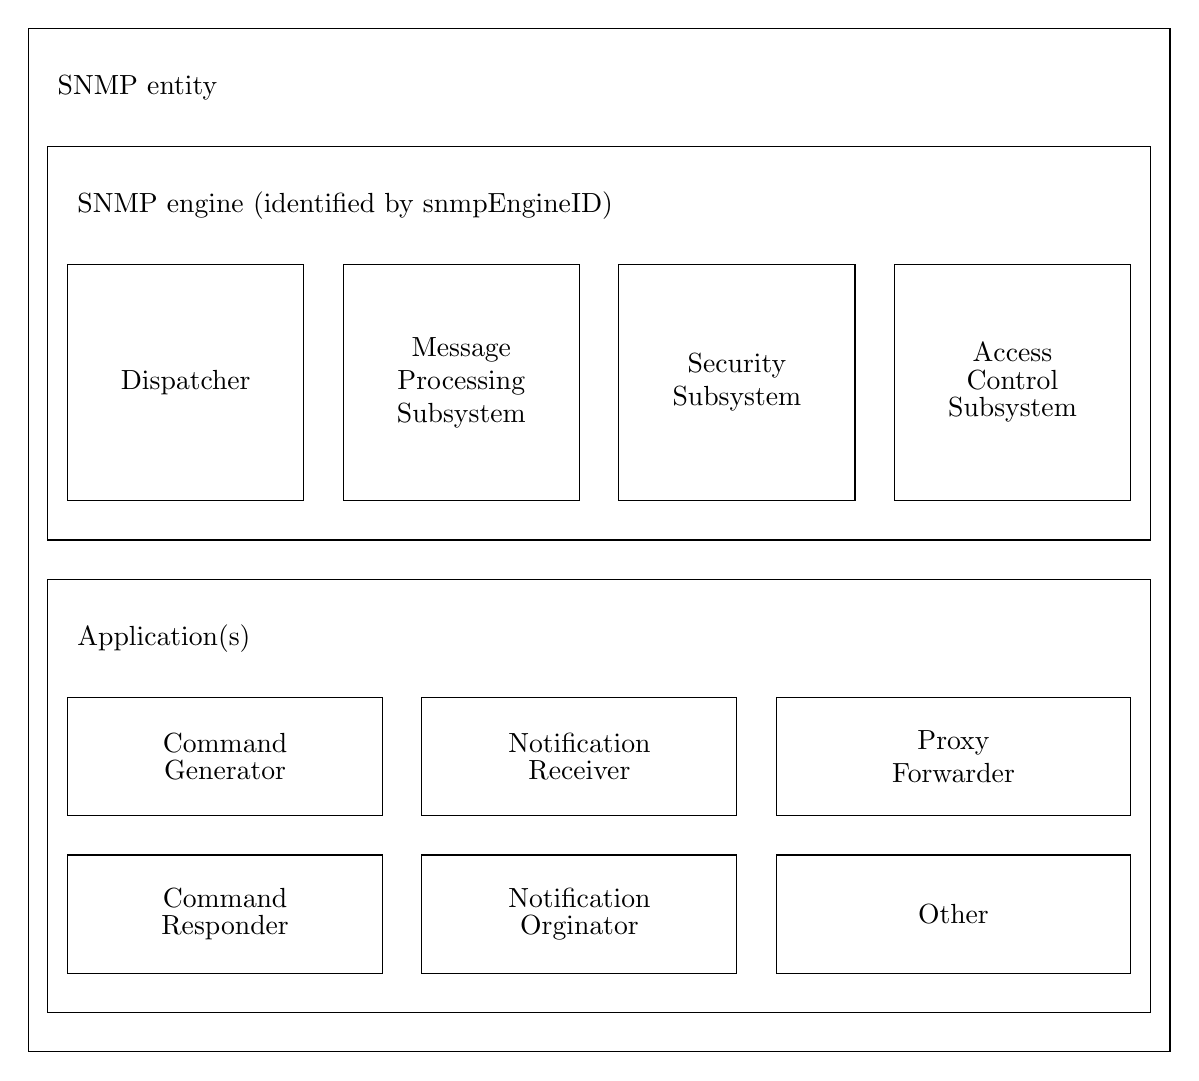
\begin{tikzpicture}
    \tikzstyle{rect} = [shape=rectangle, draw, align=center]

    \draw (0,    0) rectangle (14.5, -13) node[right] at(0.25, -0.75){SNMP entity};

        \draw (0.25, -1.5) rectangle (14.25, -6.5) node[right] at(0.5, -2.25){SNMP engine (identified by snmpEngineID)};

            \draw (0.5, -3)   rectangle (3.5, -6) node[pos=.5] {\shortstack{Dispatcher}};
            \draw (4,   -3)   rectangle (7,   -6) node[pos=.5] {\shortstack{Message\\Processing\\Subsystem}};
            \draw (7.5, -3)   rectangle (10.5,-6) node[pos=.5] {\shortstack{Security\\Subsystem}};
            \draw (11,  -3)   rectangle (14,  -6) node[pos=.5] {\shortstack{Access\\Control\\Subsystem}};

        \draw (0.25, -7) rectangle (14.25,  -12.5) node[right] at(0.5, -7.75){Application(s)};

            \draw (0.5, -8.5) rectangle (4.5, -10) node[pos=.5] {\shortstack{Command\\Generator}};
            \draw (5,   -8.5) rectangle (9,   -10) node[pos=.5] {\shortstack{Notification\\Receiver}};
            \draw (9.5, -8.5) rectangle (14,  -10) node[pos=.5] {\shortstack{Proxy\\Forwarder}};

            \draw (0.5, -10.5) rectangle (4.5,-12) node[pos=.5] {\shortstack{Command\\Responder}};
            \draw (5,   -10.5) rectangle (9,  -12) node[pos=.5] {\shortstack{Notification\\Orginator}};
            \draw (9.5, -10.5) rectangle (14, -12) node[pos=.5] {\shortstack{Other}};
\end{tikzpicture}
\caption{Naming and hierarchy of single elements from a SNMP entity (Adapted from \cite{RFC:RFC3411:2002})}
\label{Figure:SNMP-EntityNaming}
\end{figure}

The purpose of the SNMP engine is to provide services to send, receive, authenticate and encrypt messages, while also handling the access control to managed objects. For these tasks, it contains a Dispatcher, a Message Processing Subsystem, a Security Subsystem, and an Access Control Subsystem. Only one SNMP engine exists per SNMP entity. An overview of the subsystems, their naming, and hierarchy can be found in Figure \ref{Figure:SNMP-EntityNaming}.

Every SNMP engine is identified by a snmpEngineID. This identifier must be unique within an administrative domain. Because only one SNMP engine exists per SNMP entity, this identifier can also be used to identify the SNMP entity.

\newpage
The Dispatcher is used to send and receive SNMP messages. Therefore, it must be able to determine the SNMP version of a message. It provides an abstract interface for the SNMP application to send and receive messages over the network. Only one Dispatcher can exist per SNMP engine.

An SNMP engine also contains one Message Processing Subsystem, which is responsible for preparing messages for sending and extracting data from received messages. One Message Processing Subsystem can contain multiple Message Processing Models (e.g. SNMPv3, SNMPv2c, SNMPv1), whereby model processes its matching SNMP message.

The Security Subsystems is part of the SNMP engine and provides services like authentication and privacy. The subsystem may contain one or more models. Only one Security Subsystem can exist per SNMP engine.

Lastly, another subsystem included in an SNMP engine is the Access Control Subsystem, which provides one or more Access Control Models. The default Access Control Model is View-Based, only a predefined set of MIB Objects can be viewed or edited. Only one of these subsystems can exist per SNMP engine.

Figure \ref{Figure:SNMP-Manager} shows a typical setup of an SNMP Manager. It has one or more command generators and notification receivers. An instruction is generated in a command generator application and the instruction is sent to the Dispatcher. In the Dispatcher the instruction is encapsulated in a PDU. After that, the Message Dispatcher transfers the data to the Message Processing Subsystem, where the correct SNMP version and its properties are appended. The Message Processing System transfers the message to the Security Subsystem, where security-related information is added. In the next step, the message is passed to the Transport Mapping. This step adds transport-related and transport-protocol-related information to the message. After that, the message is embedded into the Transport Protocol and is delivered over the network. Receiving a message and parsing it works in reverse order. The only difference is that a notification receiver application is receiving the message instead of a command generator application. For further information, see Section 4.6.1 in RFC 3411 on page 38 \cite{RFC:RFC3411:2002}.

Figure \ref{Figure:SNMP-Agent} shows a typical setup of an SNMP Agent, which has one or more command receiver applications and notification originator applications. The process of receiving and decoding a message is the same as for an SNMP manager. After the message is decoded, it can be sent to a proxy forwarder application, which is forwarding the message to another SNMP entity, or to the notification originator application and command responder application. These applications may check if the sender is authorized to receive or write the content of the requested MIB entry. They can check if the access is granted by communicating with the access control unit. If access is granted, the content of the MIB entry may be sent back to the origin of the request in reverse order of receiving the message. For further information, see Section 4.6.2 in RFC 3411 on page 39 \cite{RFC:RFC3411:2002}.

The snmpEngineID only describes the SNMP engine and the SNMP entities. Because of that, every context (instance of MIB Objects) also needs to be uniquely identified. Every context has a readable name (e.g. bridge0, bridge1), and additionally, the contextID is provided. If the contextID is the same as the snmpEngineID, the context is only valid on this SNMP entity. If the context is valid over multiple SNMP entities, another contextID may be used, but the combination of contextName and contextID must be unique in the administrative domain. It is also possible that multiple combinations of contextID and contextName exist to identify the same object.

With SNMPv3 three levels of security have been introduced:

\begin{minipage}{\textwidth}
\begin{itemize}
    \item noAuthNoPriv - without authentication and without privacy
    \item authNoPriv - with authentication and without privacy
    \item authPriv - with authentication and with privacy
\end{itemize}
\end{minipage}

\newpage
The security levels are sorted like this: noAuthNoPriv < AuthNoPriv < AuthPriv. Every message has an associated security level and all subsystems and applications are required to provide a value of security level or to hold the same security level while processing data.

\begin{figure}[!h]
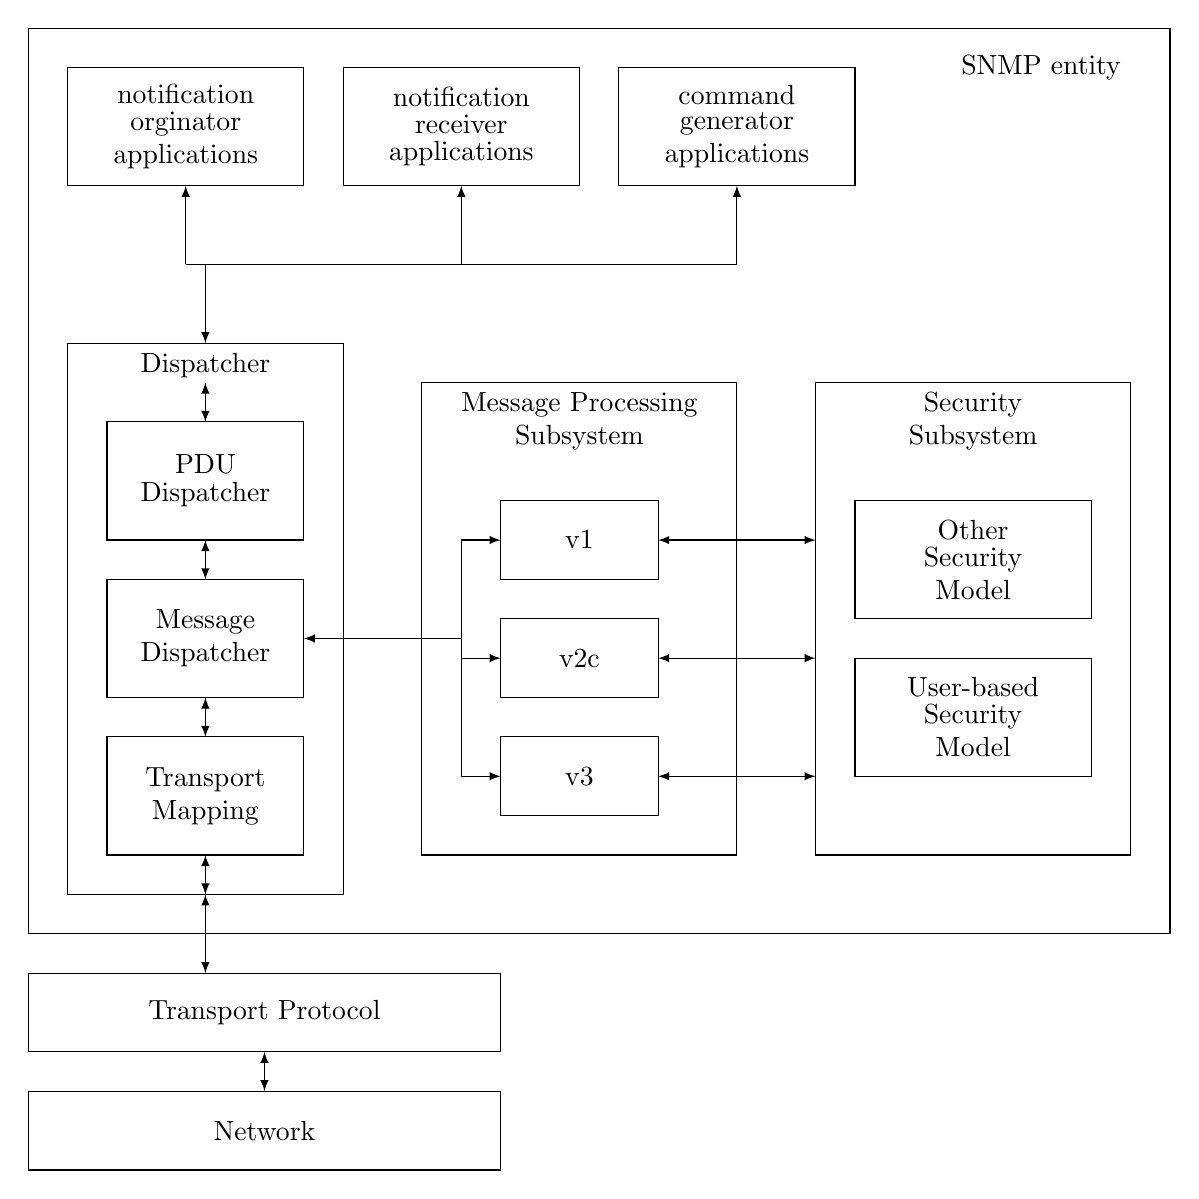
\begin{tikzpicture}
    \tikzstyle{rect} = [shape=rectangle, draw, align=center]

    \draw (0, 0) rectangle (14.5, -11.5)
        node[left] at(14, -0.5) {\shortstack{SNMP entity}};

        \draw (0.5, -0.5) rectangle ( 3.5, -2)
            node[pos=.5] {\shortstack{notification\\orginator\\applications}};
        \draw (4.0, -0.5) rectangle ( 7.0, -2)
            node[pos=.5] {\shortstack{notification\\receiver\\applications}};
        \draw (7.5, -0.5) rectangle (10.5, -2)
            node[pos=.5] {\shortstack{command\\generator\\applications}};

        \draw[latex-]   (2.0, -2) -- (2.0, -3.0);
        \draw[latex-]   (5.5, -2) -- (5.5, -3.0);
        \draw[latex-]   (9.0, -2) -- (9.0, -3.0);
        \draw[-]        (2.0, -3) -- (9.0, -3.0);
        \draw[-latex]   (2.25,-3) -- (2.25,-4.0);

        \draw (0.50, -4) rectangle (4.0, -11)
            node[below] at(2.25,-4) {\shortstack{Dispatcher}};

            \draw (1, -5) rectangle (3.5, -6.5)
                node[pos=.5] {\shortstack{PDU\\Dispatcher}};
            \draw (1, -7) rectangle (3.5, -8.5)
                node[pos=.5] {\shortstack{Message\\Dispatcher}};
            \draw (1, -9) rectangle (3.5, -10.5)
                node[pos=.5] {\shortstack{Transport\\Mapping}};

            \draw[latex-latex]  (2.25, -4.5)  -- (2.25, -5);
            \draw[latex-latex]  (2.25, -6.5)  -- (2.25, -7);
            \draw[latex-latex]  (2.25, -8.5)  -- (2.25, -9);
            \draw[latex-latex]  (2.25, -10.5) -- (2.25, -11);

        
        \draw[latex-]   (3.50, -7.75) -- (5.50, -7.75);
        \draw[-]        (5.50, -6.50) -- (5.50, -9.50);
        \draw[-latex]   (5.50, -6.50) -- (6.00, -6.50);
        \draw[-latex]   (5.50, -8.00) -- (6.00, -8.00);
        \draw[-latex]   (5.50, -9.50) -- (6.00, -9.50);


        \draw (5.00, -4.5) rectangle (9.0, -10.5)
            node[below] at(7.00, -4.5) {\shortstack{Message Processing\\Subsystem}};

            \draw (6, -6.0) rectangle (8, -7.0)
                node[pos=.5] {\shortstack{v1}};
            \draw (6, -7.5) rectangle (8, -8.5)
                node[pos=.5] {\shortstack{v2c}};
            \draw (6, -9.0) rectangle (8, -10.0)
                node[pos=.5] {\shortstack{v3}};

        \draw[latex-latex]   (8, -6.50) -- (10, -6.50);
        \draw[latex-latex]   (8, -8.00) -- (10, -8.00);
        \draw[latex-latex]   (8, -9.50) -- (10, -9.50);
        
        \draw (10.0, -4.5) rectangle (14, -10.5)
            node[below] at(12.0, -4.5) {\shortstack{Security\\Subsystem}};

            \draw (10.5, -6.0) rectangle (13.5, -7.5)
                node[pos=.5] {\shortstack{Other\\Security\\Model}};
            \draw (10.5, -8.0) rectangle (13.5, -9.5)
                node[pos=.5] {\shortstack{User-based\\Security\\Model}};

        \draw[latex-latex]  (2.25, -11)  -- (2.25, -12);

        \draw (0, -12) rectangle (6, -13)
            node[pos=.5] {\shortstack{Transport Protocol}};

        \draw[latex-latex]  (3, -13)  -- (3, -13.5);
        
        \draw (0, -13.5) rectangle (6, -14.5)
            node[pos=.5] {\shortstack{Network}};

\end{tikzpicture}
\caption{Typical structure of an SNMP manager (Adapted from \cite{RFC:RFC3411:2002})}
\label{Figure:SNMP-Manager}
\end{figure}

\begin{figure}[!h]
    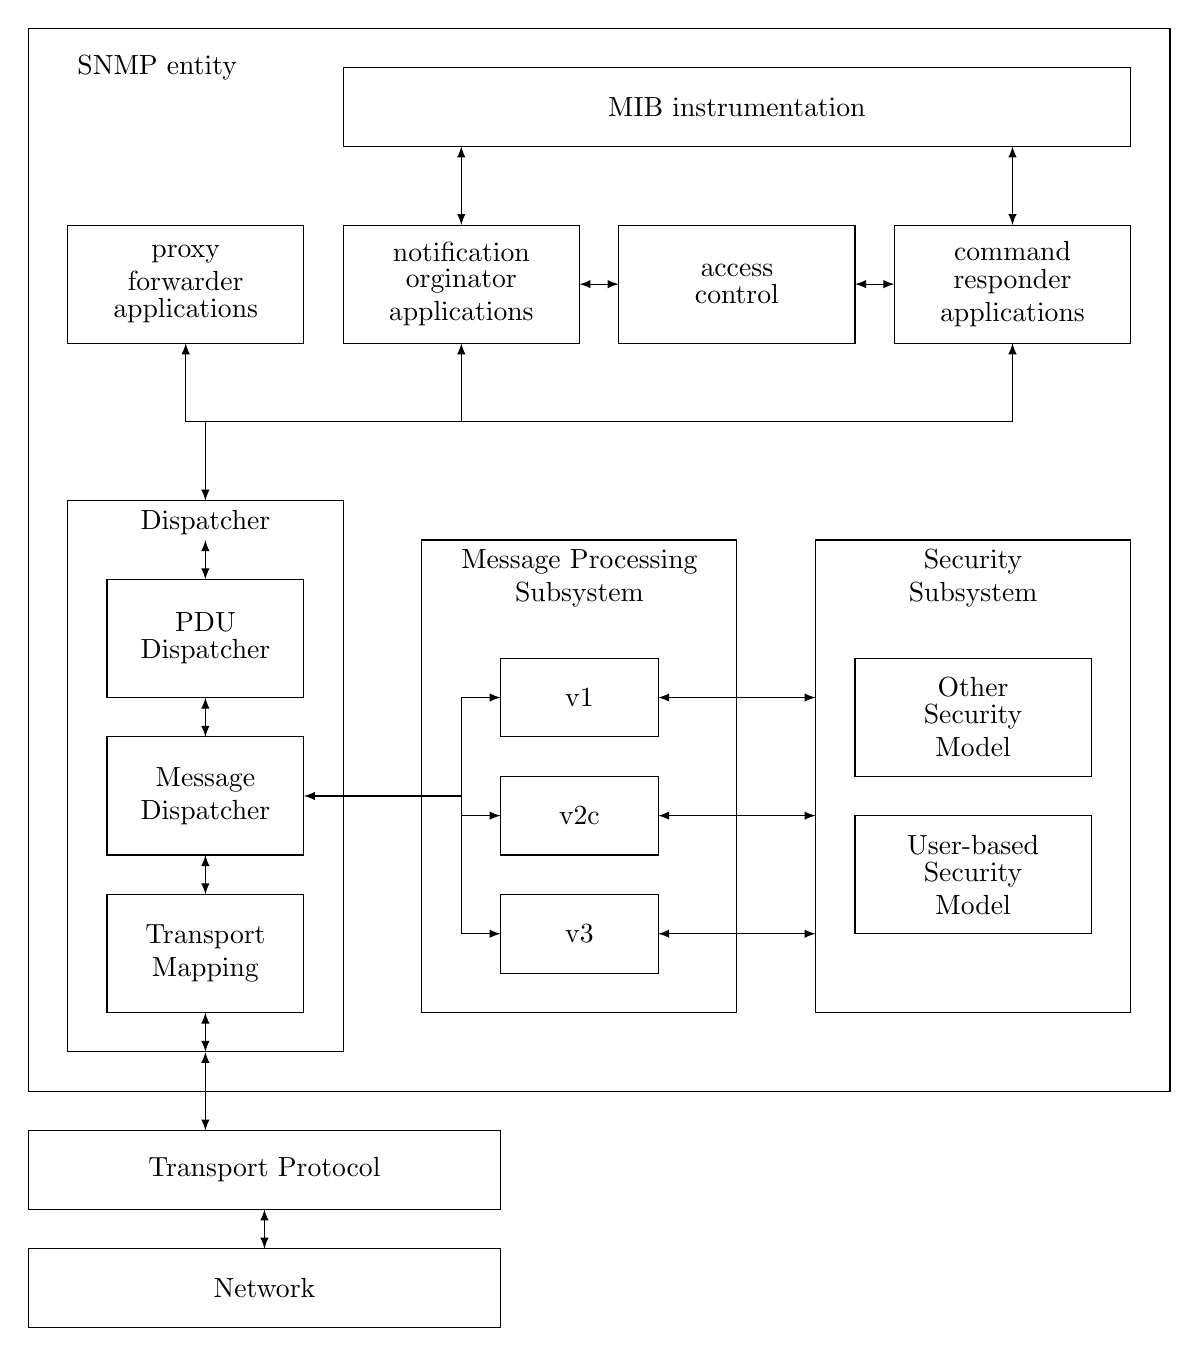
\begin{tikzpicture}
        \tikzstyle{rect} = [shape=rectangle, draw, align=center]
    
        \draw (0, 2) rectangle (14.5, -11.5)
            node[right] at(0.5, 1.5) {\shortstack{SNMP entity}};
    
            \draw (4, 1.5) rectangle (14, 0.5)
                node[pos=.5] {\shortstack{MIB instrumentation}};
    
            \draw[latex-latex]   (5.5, 0.5) -- (5.5, -0.5);
            \draw[latex-latex]   (12.5,0.5) -- (12.5,-0.5);
    
            \draw (0.5, -0.5) rectangle ( 3.5, -2)
                node[pos=.5] {\shortstack{proxy\\forwarder\\applications}};
            \draw (4.0, -0.5) rectangle ( 7.0, -2)
                node[pos=.5] {\shortstack{notification\\orginator\\applications}};
            \draw (7.5, -0.5) rectangle (10.5, -2)
                node[pos=.5] {\shortstack{access\\control}};
            \draw (11,  -0.5) rectangle (14, -2)
                node[pos=.5] {\shortstack{command\\responder\\applications}};
    
            \draw[latex-latex]   (10.5, -1.25) -- (11,  -1.25);
            \draw[latex-latex]   (7.0,  -1.25) -- (7.5, -1.25);
    
            \draw[latex-]   (2.0, -2) -- (2.0, -3.0);
            \draw[latex-]   (5.5, -2) -- (5.5, -3.0);
            \draw[latex-]   (12.5,-2) -- (12.5,-3.0);
            \draw[-]        (2.0, -3) -- (12.5,-3.0);
            \draw[-latex]   (2.25,-3) -- (2.25,-4.0);
    
            \draw (0.50, -4) rectangle (4.0, -11)
                node[below] at(2.25,-4) {\shortstack{Dispatcher}};
    
                \draw (1, -5) rectangle (3.5, -6.5)
                    node[pos=.5] {\shortstack{PDU\\Dispatcher}};
                \draw (1, -7) rectangle (3.5, -8.5)
                    node[pos=.5] {\shortstack{Message\\Dispatcher}};
                \draw (1, -9) rectangle (3.5, -10.5)
                    node[pos=.5] {\shortstack{Transport\\Mapping}};
    
                \draw[latex-latex]  (2.25, -4.5)  -- (2.25, -5);
                \draw[latex-latex]  (2.25, -6.5)  -- (2.25, -7);
                \draw[latex-latex]  (2.25, -8.5)  -- (2.25, -9);
                \draw[latex-latex]  (2.25, -10.5) -- (2.25, -11);
            
            \draw[latex-]   (3.50, -7.75) -- (5.50, -7.75);
            \draw[-]        (5.50, -6.50) -- (5.50, -9.50);
            \draw[-latex]   (5.50, -6.50) -- (6.00, -6.50);
            \draw[-latex]   (5.50, -8.00) -- (6.00, -8.00);
            \draw[-latex]   (5.50, -9.50) -- (6.00, -9.50);
    
    
            \draw (5.00, -4.5) rectangle (9.0, -10.5)
                node[below] at(7.00, -4.5) {\shortstack{Message Processing\\Subsystem}};
    
                \draw (6, -6.0) rectangle (8, -7.0)
                    node[pos=.5] {\shortstack{v1}};
                \draw (6, -7.5) rectangle (8, -8.5)
                    node[pos=.5] {\shortstack{v2c}};
                \draw (6, -9.0) rectangle (8, -10.0)
                    node[pos=.5] {\shortstack{v3}};
    
            \draw[latex-latex]   (8, -6.50) -- (10, -6.50);
            \draw[latex-latex]   (8, -8.00) -- (10, -8.00);
            \draw[latex-latex]   (8, -9.50) -- (10, -9.50);
            
            \draw (10.0, -4.5) rectangle (14, -10.5)
                node[below] at(12.0, -4.5) {\shortstack{Security\\Subsystem}};
    
                \draw (10.5, -6.0) rectangle (13.5, -7.5)
                    node[pos=.5] {\shortstack{Other\\Security\\Model}};
                \draw (10.5, -8.0) rectangle (13.5, -9.5)
                    node[pos=.5] {\shortstack{User-based\\Security\\Model}};
    
            \draw[latex-latex]  (2.25, -11)  -- (2.25, -12);
    
            \draw (0, -12) rectangle (6, -13)
                node[pos=.5] {\shortstack{Transport Protocol}};
    
            \draw[latex-latex]  (3, -13)  -- (3, -13.5);
            
            \draw (0, -13.5) rectangle (6, -14.5)
                node[pos=.5] {\shortstack{Network}};
    
    \end{tikzpicture}
    \caption{Typical structure of a SNMP agent (Adapted from \cite{RFC:RFC3411:2002})}
    \label{Figure:SNMP-Agent}
    \end{figure}

\newpage
~\newpage

\subsection{Protocol}
\label{Section:SNMP-Protocol}
The basic functions of the protocol are defined in RFC3416 \cite{RFC:RFC3416:2002}. It is defined that it should be possible to retransmit a request. Under normal circumstances, the receiver is required to send a response to the originator of the message. If no response is received, the originator can decide if the message should be retransmitted, but the application needs to act responsibly with the retransmission frequency and duration.

The message size is limited to the capabilities of all SNMP entities that are part of the communication. The maximum size of a message is defined by the smallest value of the maximum size that both the receiving SNMP entity can accept and the sending SNMP entity can generate. The maximum size an entity can receive may be known. Otherwise the size is defined by the transport domain when sending the message. The maximum size an entity can generate is defined by local constraints. Each transport mapping defines a minimum size, which every entity needs to be able to consume and produce.

The goal of the GetBulkRequest-PDU is to reduce the number of messages. Therefore, messages should be as large as possible. To achieve this, the PDU is embedding the limits of supported message sizes from the command responder and command generator into the request. It can happen that the maximum message size is bigger than the MTU of the network, leading to fragmentation of the message. Message fragmentation can decrease the reliability of the transfer.

SNMP only requires an unreliable datagram. The protocol encourages the use of UDP to send messages, but other transport mappings can also be used.

PDUs contain a request-id field. The request-id is generated by the sending SNMP entity and added to the Request-PDU. If a response for that request is sent by the receiving entity, the request-id from the received request is used. This makes it easy to match sent requests with the incoming response.  To calculate round-trip time, the request-id needs to be changed if the PDU is retransmitted. A non-zero value of the error-status field in the Response-PDU indicates that an error occurred. The error-index field represents which variable-binding caused the error. Thereby, the error-index is the same as the index of the variable-binding in a variable-binding list.

The different PDUs can contain fields that are not relevant for the specific PDU type. These fields are ignored while processing the PDU by the receiving entity. Every field, even the ignored ones, must have a valid ASN.1(\ref{Section:MIB-Syntax}) syntax and encoding. There can be as many variable bindings as fit into the message size limit, but no more than 21474483647.

\newpage
The GetRequest-PDU is generated and is transmitted by the request of an application. Each variable binding in the variable-binding list is getting processed by the receiving SNMP entity. Every field of the Response-PDU has the same value as the corresponding sent PDU. They are processed as follows: If the variable name exactly matches the name of the accessible variable, then the variable field is set to the value of the accessible variable.  If the name does not match exactly and does not have an OID prefix that matches the requested OID prefix, the value is set to "noSuchObject". Otherwise, the variable field is set to "noSuchInstance".

If any other error occurs, the Response-PDU is set to the same value as the received fields and the error-status field is set to "genError". Otherwise, the error-status field is set to "noError" and the error-index field is set to zero. If the message is shorter than or equals the maximum message size, the Response-PDU is transmitted to the originator. Otherwise, an alternative Response-PDU is generated, with the same values as the received PDU, the error-status field set to "tooBig" and the error-index field set to 0. If this alternate Response-PDU is bigger than the maximal message size, the message is dropped and the snmpSilentDrops counter is increased.

The GetNextRequest-PDU is generated and is transmitted by the request of an application. The variables are processed as follows: The successor variable of the lexicographically order variable names is located. The found name and the value are set in the Response-PDU to the same index as the variable of the GetNextRequest-PDU. If the requested variable has no successor, then the value is set to "endOfMibView" and the name is set to the name of the variable from the GetNextRequest-PDU. The errors are handled in the same way as for the GetRequest-PDU.

The GetBulkRequest-PDU is generated and transmitted by the request of an application. The purpose of this PDU is to request a large amount of data, but it also can be used to retrieve large tables rapidly and efficiently. Every variable is processed on receive and a Responds-PDU is produced with the request-id, but the variables are not mapped one-to-one like in the GetRequest-PDU, GetNextRequest-PDU, and SetRequest-PDU. This PDU has a non-repeaters and max-repetitions field, which is not included in other PDUs. The non-repeaters field contains the number of variables in the variable list where a single-lexicographic successor can be returned, while the max-repetitions field contains the number of lexicographic successors for the remaining variables.

In the following description, we define these variables: $N$ is the value of the non-repeaters field, $M$ is the value of the max-repetitions field, and $R$ is the maximum of variables minus the value of non-repeater fields $N$. The variables get requested as follows: One variable of the Respond is assigned to the first $N$ variables, $M$ variables are requested for the $R$ variables. This results in a total number of $N + (M * R)$ requests. A more detailed explanation is given in RFC 3416 Section 4.2.3 on page 15 \cite{RFC:RFC3416:2002}. The errors are handled the same as for the GetRequest-PDU.

\newpage
The SetRequest-PDU is generated and is transmitted by the request of an application. The receiving entity parses the PDU and produces a response PDU. In the first step, the variables are validated, and if all validations succeed, the variables get altered. These validations are performed:

\begin{itemize}
    \item Access for the variable name is validated. If no access is granted, the error-status is "noAccess".
    \item If the OID prefix does not match any variable that can be created or modified, the error-status is set to "notWriteable".
    \item If the ASN.1 type is inconsistent with the required type, the error-status is set to "wrongType"
    \item If the required length is inconsistent, the error-status is set to "wrongLength"
    \item If the encoding does not match ASN.1, the error-status is set to "wrongEncoding"
    \item If a value is specified that can not be set, the error-status is set to "wrongValue".
    \item If a specified variable does not exist or can not be created, the error-status is set to "noCreation".
    \item If a specified variable does not exist and can not be created under circumstances, the error-status is set to "inconsistentName".
    \item If a variable is specified that can not be created or modified, no matter of the new value, the error-status is set to "notWriteable".
    \item If a value can not be set or modified, but is getting modified, the error-status is set to "inconsistentValue".
    \item If the variable needs allocation of a resource that is not available, the error-status is set to "resourceUnavailable".
    \item If the processing fails for another reason, the error-status is set to "genErr".
\end{itemize}

If a requested variable does not exist, it is created and the value is assigned to it. When the same variable should be set multiple times with different values in one request, the behavior is implementation-specific. If an assignment fails, all other assignments from the same request get reverted and the error-status is set to "commitFailed". If it is not possible to revert all assignments, the error-status is set to "undoFailed". It is recommended for implementations to avoid both cases.

\newpage
The SNMPv2-Trap-PDU is generated and is transmitted on behalf of a notification originator application. These PDUs are often used to inform remote entities about events that occurred. The PDUs are not getting confirmed and the destinations for these PDUs are implementation-dependent. The first variables in an SNMPv2-Trap-PDU are sysUpTime.0 and snmpTrapOID.

The InformRequest-PDU is generated and is transmitted on behalf of a notification originator application. Like SNMPv2-Trap, it informs about an event without guarantee of delivery, but adds confirmation. The destination to which it is sent is defined by the notification originator. The first two variables in the PDU are sysUpTime.0 and snmpTrapOID. If an InformRequest-PDU is received, the entity validates the received PDU. If the validation succeeds, the entity presents its content to the appropriate application, generates a Respond-PDU to confirm the PDU, and transmits it.

\subsection{Transport Subsystem}
\label{Section:SNMP-TransportSubsystem}

The goal of the Transport Subsystem (\cite{RFC:RFC5590:2009}) is to provide access to lower-layer security mechanisms. This can include authentication of the sender, encryption, data integrity, and timeliness checking. Examples for these techniques are TLS, Simple Authentication and Security Layer (SASL) as well as SSH. Transport Mappings need to use security protocols the way they were designed. Modified usage often implies that the protocol can not deliver the expected security characteristics. They also should not modify the underlying security protocol, which might change it is security characteristics.

Transport Subsystems must meet the following requirements:
\begin{itemize}
    \item They must follow the architectural modularity requirements.
    \item If establishing the connection between two entities for every message is too expensive, sessions can be used.
    \item The security model must use the same or a higher security level than provided by the transport model.
    \item A message processing model might unpack security-specific parameters from incoming messages, before calling a specific security model.
    \item Authentication and authorization are separated. Authentication is handled by the security model and authorization by the access control model.
\end{itemize}

A security name is a human-readable value, that describes the used security protocol and is used by SNMP applications and the Access Control Subsystem. The transport mapping security name is a human-readable value and is used by the transport and security models to identify the used transport security protocol.

\newpage
The security value consists of two values: the requested security level, and the transport security level. The first value represents the minimum security level required for transport models. It can be used to prevent sending messages via sessions that are not secure enough. The second value represents the security level offered by the session. The security model can use this to ensure the minimum security level for incoming messages for a session.

\subsection{Transport Mapping}
\label{Section:SNMP-TransportMapping}

Transport Mappings are used to describe the way how data is transferred between multiple SNMP entities. An SNMP entity can use multiple transport mappings, but every entity should provide access via UDP over IPv4. If an entity supports IPv4 as Transport Mapping, it must also implement UDP over IPv4. The definition for Transport Mappings can be found in RFC 3417 \cite{RFC:RFC3147:2002}.

It should be mentioned that popular Transport Mappings are "SNMP over UDP over IPv4" \cite{RFC:RFC3147:2002}, "SNMP over UDP over IPv6" \cite{RFC:RFC3147:2002} and "SNMP over IEEE 802 Networks (Ethernet)" \cite{RFC:RFC4789:2006}. To be able to communicate with SNMPv1 entities, a proxy is needed \cite{RFC:RFC2576:2000}. 